Previo a cualquier configuracion o funcion a llamar dentro de nuestro kernel, se llamo a la instruccion CLI, la cual nos deshabilito las interrupciones ("saltando a modo protegido"). Una vez deshabilitadas y en modo protegido, establecimos la tabla de interrupciones con la instruccion LIDT. A esta instruccion le pasamos la tabla ya configurada, con las interrupciones posibles: tanto las excepciones como las interrupciones. Cada entrada fue configurada para ser ejecutada en el segmento de codigo de kernel (selector 0x90), ya que el debe ser el responsable de ellas. Las rutinas de atencion, configuradas en el offset de cada descriptor de la IDT, notifican al context manager el evento producido, para que este actualice los datos en los distintos modulos: sea pantalla o mmu. 

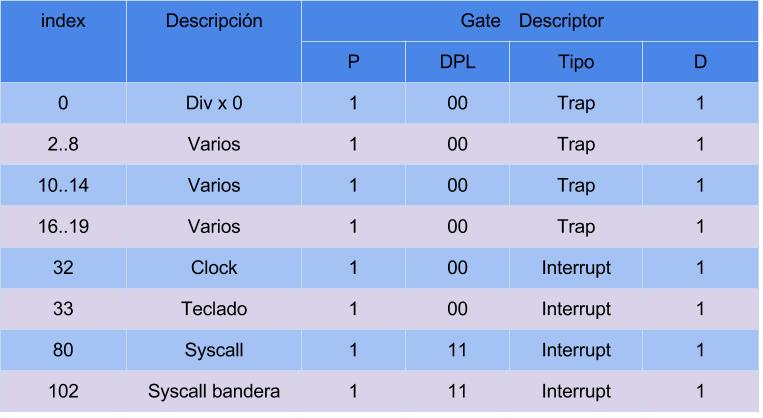
\includegraphics[scale=0.4]{diagramas/idt.jpg}
\\Descriptores de la IDT.\\

Los campos de offset se completaron con la direccion de los handlers de atencion a las interrupciones, en donde dependiendo del tipo, se recurre a distintos modulos para resolver el evento producido.\\

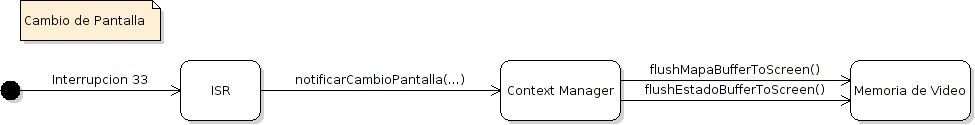
\includegraphics[scale=0.4]{diagramas/cambioPantalla-handler.jpg}
\\\centering{Manejador de cambio de pantalla}\\
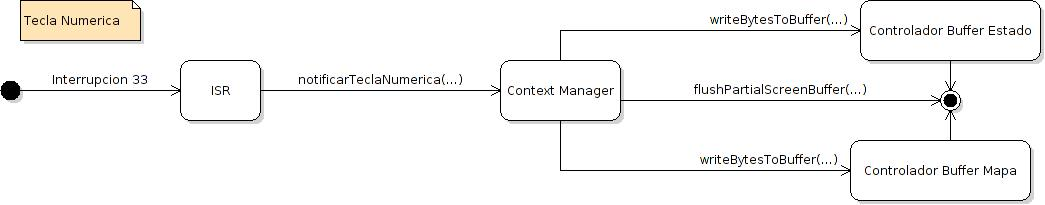
\includegraphics[scale=0.4]{diagramas/teclaNumerica-handler.jpg}
\\\centering{Interrupcion por tecla num\'erica}\\
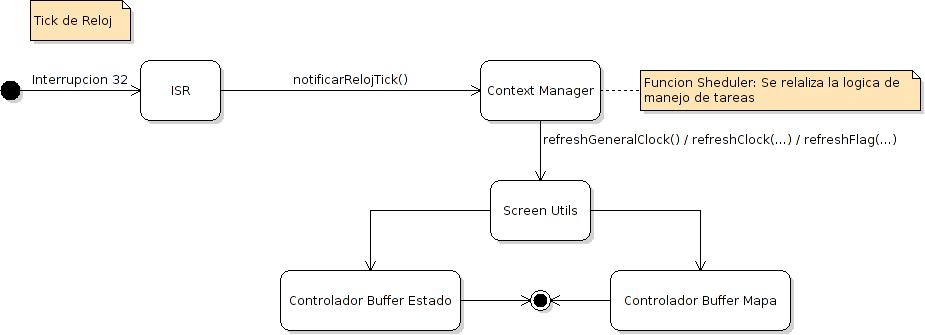
\includegraphics[scale=0.4]{diagramas/tickReloj-handler.jpg}
\\\centering{Interrupcion del clock}\\
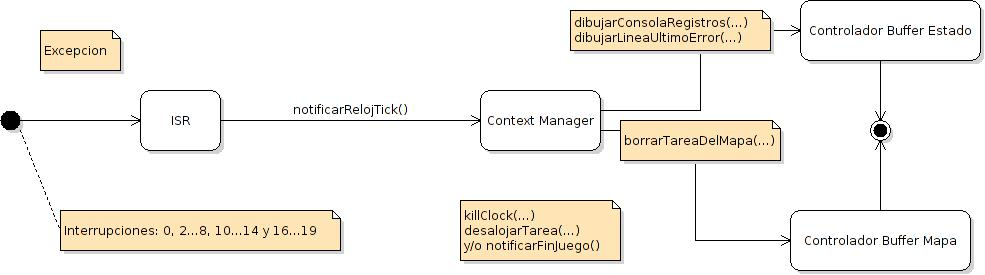
\includegraphics[scale=0.4]{diagramas/excepcion-handler.jpg}
\\\centering{Manejo de las excepci\'ones}\\
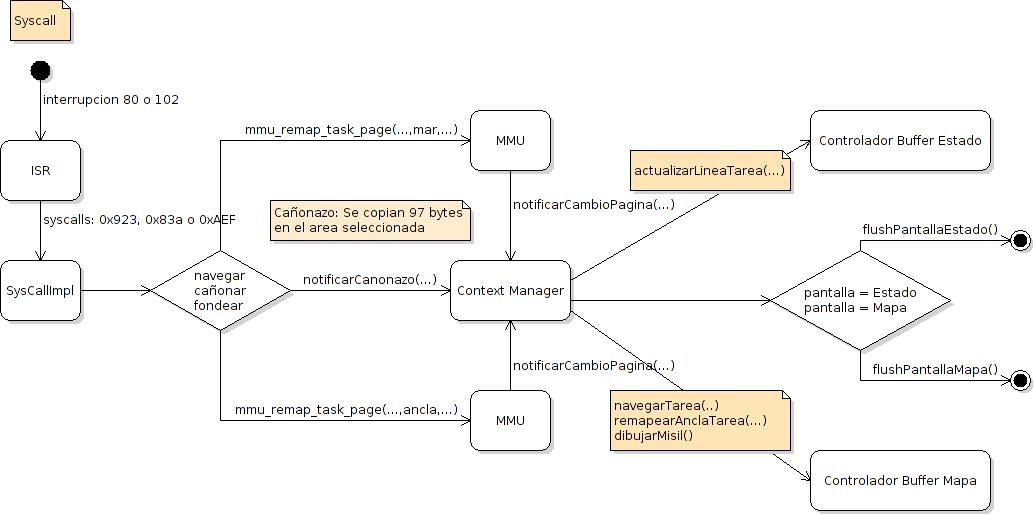
\includegraphics[scale=0.4]{diagramas/syscall-handler.jpg}
\\\centering{Llamadas al sistema}\\



